\chapter{\leavevmode\newline The Standard Model of Particle Physics}
\label{chap:chapter_1}
Several particles were discovered after years of experimental observations, and this led to the development of the Standard Model (SM) during the 1970s. The SM does not only describe the fundamental particles and interactions (except for gravitation) but also predicts new particles. The fundamental particles in the SM have a property known as spin and are divided into two main groups, Fermions, and Bosons, as shown in Fig \ref{fig:sm}.

Fermions obey the Pauli exclusion principle, have half-integer spin, and there exists an antiparticle with the same properties but opposite quantum numbers, such as electric charge. They are subdivided into Quarks and Leptons, both groups having six particles, and they are further grouped into three generations according to their mass. Quarks ($u, d, s, c, t, b$) are always found in bound states known as hadrons. A bounded state of a quark and an antiquark forms a meson, while three bounded quarks form a baryon. Leptons on the other hand have integer spin and are electrically charged (e, $\mu$, $\tau$) or neutral (their corresponding neutrinos, $\nu_e, \nu_\mu, \nu_\tau$).

Bosons are known as the force or interaction carriers and are divided into vector and scalar bosons. The scalar boson is the Higgs boson, and it gives the other elementary particles mass. The vector bosons are related to the fundamental interactions. The photon is the electromagnetic interaction carrier, the massive bosons, $W^{\pm}$ and $Z$, mediate the weak force and gluons the strong force. The theory that describes the strong force is known as Quantum Chromodynamics (QCD) and will be briefly discussed in the next section.

SM is considered the most successful theory developed by mankind, however, there are several physical phenomena it cannot explain. For instance, the existence of three and only three generations of fermions. It does not account for gravity and to date, there is no observation of the vector boson responsible for the gravitational interaction, also known as the graviton. It also does not describe why there is more matter than antimatter in the universe, among other properties.

A more complete description of the model requires the understanding of the underlying Quantum Field Theory (QFT) in which SM is based, and the symmetries of the Lie group SU(3)$ \times$ SU(2)$ \times$ U(1).

\begin{figure}[htp!]
	\centering
	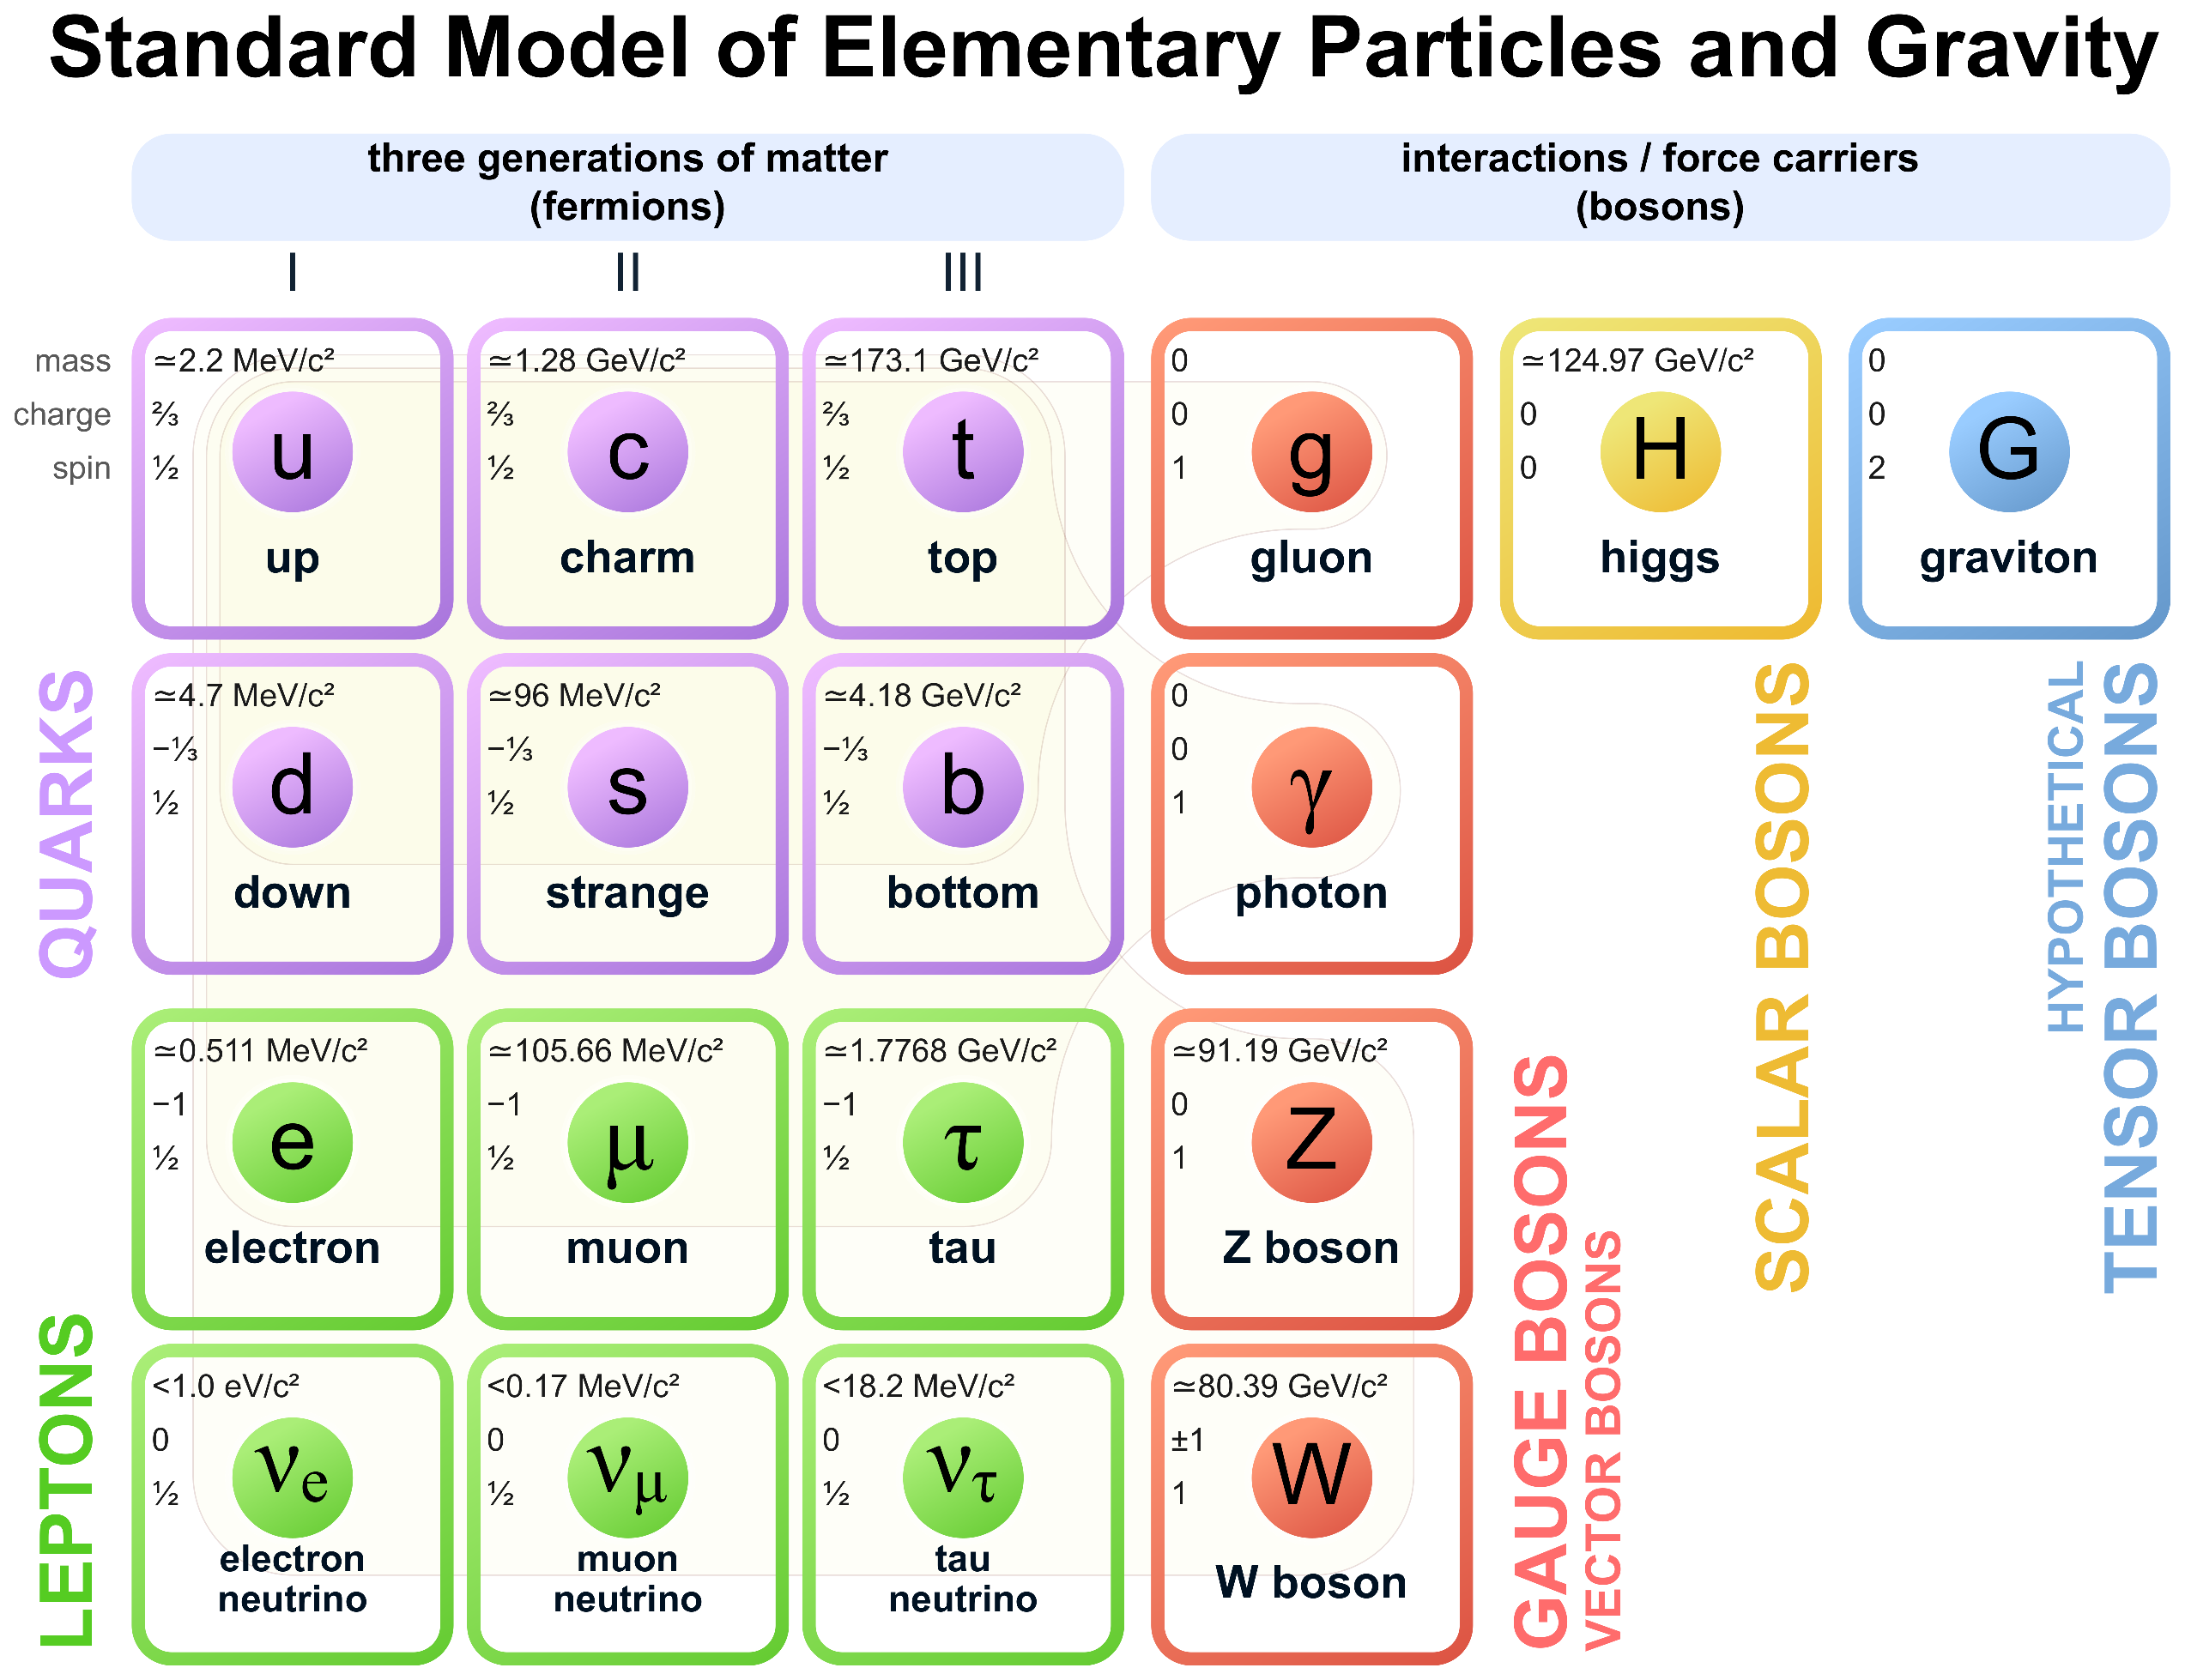
\includegraphics[scale=0.34]{MainContent/Figs/SM.eps}
	\caption{The Standard Model of fundamental particles. Retrieved from}
	\label{fig:sm}
\end{figure}

\section{QCD}
\section{$B^0_s$}
\subsection{$B^0_s \to J/\psi\phi$}
